\documentclass{article}
\usepackage[utf8]{inputenc}
\usepackage{geometry}
\usepackage{graphicx}
\usepackage{amsmath}
\usepackage{amsfonts}
\usepackage{amsthm}
\usepackage{amssymb}
\usepackage[most]{tcolorbox}
\usepackage{array}
\usepackage{latexsym}
\usepackage{alltt}
\usepackage{hyperref}
\usepackage{color}
\usepackage{float}
\usepackage{pdfpages}
\usepackage{algpseudocode}
\usepackage{multicol}
\usepackage{multirow}
\usepackage{caption}
\usepackage{xparse}
\usepackage{setspace}
\usepackage{enumitem}
\usepackage{pdflscape}
\usepackage{parskip}

\usepackage{blindtext}
\usepackage{forest}

% \usepackage{qtree} % For \Tree

\geometry
{
  a4paper,
  left=12mm,
  right=12mm,
  top=12mm,
  bottom=15mm,
}

% mybox
\newtcolorbox{mybox}[3][]
{
  colframe = #2!25,
  colback  = #2!10,
  coltitle = #2!20!black,  
  title    = {#3},
  #1,
}

% New environments that use mybox
\newcounter{example}[section]
\newenvironment{example}[1]{\begin{mybox}[breakable]{green}{\refstepcounter{example}\textbf{Example \thesection.\theexample #1}}}{\end{mybox}}

\newcounter{definition}[section]
\newenvironment{definition}[1]{\refstepcounter{definition}\begin{mybox}[breakable]{blue}{\textbf{Definition \thesection.\thedefinition #1}}}{\end{mybox}}

\newcounter{theorem}[section]
\newenvironment{theorem}[1]{\begin{mybox}{red}{\refstepcounter{theorem}\textbf{Theorem \thesection.\thetheorem #1}}}{\end{mybox}}

\newenvironment{formula}[1]{\begin{mybox}{cyan}{\textbf{#1}}}{\end{mybox}}

% Changing maketitle
\makeatletter         
\renewcommand\maketitle{
{\raggedright % Note the extra {
\begin{center}
{\Large \bfseries \@title}\\[2ex] 
{\large \@author \ - \@date}\\[2ex]
\end{center}}} % Note the extra }
\makeatother

% \onehalfspacing % adjust spacing
\setlength{\parskip}{0.5\baselineskip}

% macros
\newcommand{\prob}[1]{\textbf{\textit{P}}\left\{#1\right\}}
\newcommand{\expc}[1]{\mathbf{E}\left(#1\right)}
\newcommand{\expcs}[1]{\mathbf{E}^2\left(#1\right)}
\newcommand{\var}[1]{\text{Var}\left( #1 \right)}
\newcommand{\ra}{\rightarrow}
\newcommand{\Ra}{\Rightarrow}

\NewDocumentCommand{\dsum}{%
    e{^_}
}{%
  {% 
    \displaystyle\sum
    \IfValueT{#1}{^{#1}}
    \IfValueT{#2}{_{#2}}
  }
}%

% maketitle variables
\title{CENG 280 - HW2}
\author{Burak Metehan Tunçel}
\date{\today}

\begin{document}

\section*{Student Information}

\textbf{Name:} Burak Metehan Tunçel

\textbf{ID:} 2468726

\section*{Answer 1}

\subsection*{a)}

% Write a context-free grammar for the language $L_1 = \left\{ w\ |\ w \in \left\{ a, b \right\}^* \land w \textnormal{ has twice as many $b$'s as $a$'s} \right\}$

\begin{equation*}
  G_1 = \left( V_1, \Sigma_1, R_1, S_1 \right)
\end{equation*}
with
\begin{multicols}{3}
  \begin{itemize}
    \vspace*{\fill}
    \item[] $V_1 = \left\{ S_1, a, b \right\}$
    \vspace*{\fill}

    \columnbreak
    
    \vspace*{\fill}
    \item[] $\Sigma_1 = \left\{ a, b \right\}$
    \vspace*{\fill}
    
    \columnbreak
    
    \vspace*{\fill}
    \item[] $R_1 = \left\{
    \begin{aligned}
      &S_1 \ra S_1bS_1bS_1aS_1,\\
      &S_1 \ra S_1bS_1aS_1bS_1,\\
      &S_1 \ra S_1aS_1bS_1bS_1,\\
      &S_1 \ra e
    \end{aligned} \right\}$
    \vspace*{\fill}
  \end{itemize}
\end{multicols}


\subsection*{b)}

% Write a context-free grammar for the language $L_2 = \left\{ a^nb^m\ |\ m,n \in \mathbb{N} \land m \leq n \leq 2m \right\}$

\begin{equation*}
  G_2 = \left( V_2, \Sigma_2, R_2, S_2 \right)
\end{equation*}
with
\begin{multicols}{3}
  \raggedcolumns
  \centering
  \begin{itemize}
    \vspace*{\fill}
      \item[] $V_2 = \left\{ S_2, a, b \right\}$
    \vspace*{\fill}

    \columnbreak
    
    \vspace*{\fill}
      \item[] $\Sigma_2 = \left\{ a, b \right\}$
    \vspace*{\fill}
    
    \columnbreak

    \vspace*{\fill}
      \item[] $R_2 = \left\{
        \begin{aligned}
          &S_2 \ra aS_2b,\\
          &S_2 \ra aaS_2b,\\
          &S_2 \ra e
        \end{aligned} \right\}$
    \vspace*{\fill}
  \end{itemize}
\end{multicols}





\subsection*{c)}

% Formally define and draw a PDA that accepts $L_1$
\begin{multicols}{2}
  
Let
\begin{equation*}
  M_1 = \left( \{p, q\}, \Sigma_1, V_1, \Delta, p, \{q\} \right)
\end{equation*}
where, $\Delta$ contains the following transitions
\begin{center}
  $\Delta = \left\{ 
    \begin{aligned}
      &((p, e, e), (q, S_1)),\\
      &((q, e, S_1), (q, S_1bS_1bS_1aS_1)),\\
      &((q, e, S_1), (q, S_1bS_1aS_1bS_1)),\\
      &((q, e, S_1), (q, S_1aS_1bS_1bS_1)),\\
      &((q, e, S_1), (q, e)),\\
      &((q, a, a), (q, e)),\\
      &((q, b, b), (q, e)),
    \end{aligned}
    \right\}$
\end{center}

\vfill\null
\columnbreak

PDA that accepts the $L_1$:
\begin{center}
  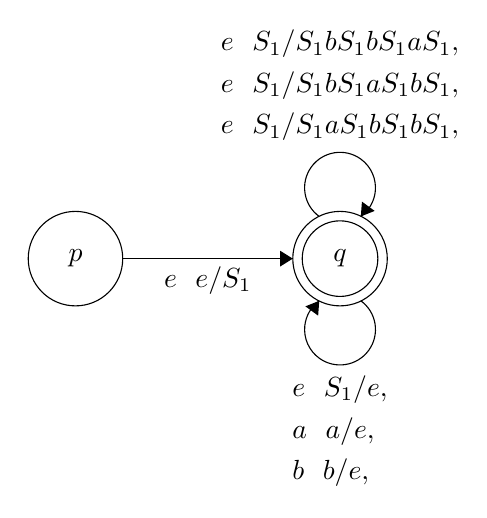
\begin{tikzpicture}[scale=0.2]
  \tikzstyle{every node}+=[inner sep=0pt]
  \draw [black] (3.2,-9.1) circle (3);
  \draw (3.2,-9.1) node {$p$};
  \draw [black] (20,-9.1) circle (3);
  \draw (20,-9.1) node {$q$};
  \draw [black] (20,-9.1) circle (2.4);
  \draw [black] (6.2,-9.1) -- (17,-9.1);
  \fill [black] (17,-9.1) -- (16.2,-8.6) -- (16.2,-9.6);
  \draw (11.6,-9.6) node [below] {$e\ \ e/S_1$};
  \draw [black] (18.677,-6.42) arc (234:-54:2.25);
  \draw (20,-1.85) node [above] {
    $\begin{aligned}
      &e\ \ S_1 / S_1bS_1bS_1aS_1,\\
      &e\ \ S_1 / S_1bS_1aS_1bS_1,\\
      &e\ \ S_1 / S_1aS_1bS_1bS_1,\\
      \end{aligned}$};
  \fill [black] (21.32,-6.42) -- (22.2,-6.07) -- (21.39,-5.48);
  \draw [black] (21.323,-11.78) arc (54:-234:2.25);
  \draw (20,-16.35) node [below] {
    $\begin{aligned}
      &e\ \ S_1 / e,\\
      &a\ \ a / e,\\
      &b\ \ b / e,
    \end{aligned}$};
  \fill [black] (18.68,-11.78) -- (17.8,-12.13) -- (18.61,-12.72);
  \end{tikzpicture}
\end{center}

\end{multicols}

\newpage
\subsection*{d)}

% Write a context-free grammar for the language $L_3 = L_1 \cup L_2$

Let $S$ be a new symbol and let $G_3 = \left( V_3, \Sigma_3, R_3, S \right)$
where
\begin{itemize}
  \item $V_3 = V_1 \cup V_2 \cup \{ S \} = \{ S_1, S_2, S, a, b \}$
  \item $\Sigma_3 = \Sigma_1 \cup \Sigma_2 = \{ a, b \}$
  \item $R_3 = R_1 \cup R_2 \cup \left\{ S \ra S_1, S \ra S_2 \right\} 
    = \left\{  
      \begin{aligned}
        S &\ra S_1, & S &\ra S_2,\\
        S_1 &\ra S_1bS_1bS_1aS_1, & S_1 &\ra S_1bS_1aS_1bS_1,\\
        S_1 &\ra S_1aS_1bS_1bS_1, & S_1 &\ra e,\\
        S_2 &\ra aS_2b, & S_2 &\ra aaS_2b,\\
        S_2 &\ra e
      \end{aligned} 
    \right\}$
\end{itemize}

The only rules involving $S$ are $S \ra S_1$ and $S \ra S_2$, so $S \Ra_G^* w$ if and only if either $S_1 \Ra_{G_1}^* w$ or $S_2 \Ra_{G_2}^* w$. Also, since $G_1$ and $G_2$ have disjoint sets of nonterminals, the last disjunction is equivalent to saying that $w \in L(G_1) \cup L(G_2)$.



\section*{Answer 2}

% Given $G_1 = \{ V, \Sigma, R, S \}$ where $V = \{ 0, 1, S, A \}, \Sigma = \{ 0, 1 \}$, and $R = \{ S \ra AS\ |\ e, A \ra A1\ |\ 0A1\ |\ 01 \}$

\subsection*{a)}

% Show that $G_1$ is ambiguous.

One way to show $G_1$ i ambiguous is showing that there are more than 1 derivations or parse tree for string $w$ such that $w \in L(G_1)$. For example, there are more than 1 derivations for $w = 00111$:
\begin{table}[ht]
  \centering
  \begin{tabular}{ccccccccccc}
    $S$ & $\Ra$ & $AS$ & $\Ra$ & $0A1S$ & $\Ra$ & $0A11S$ & $\Ra$ & $00111S$ & $\Ra$ & $00111$\\
    $S$ & $\Ra$ & $AS$ & $\Ra$ & $A1S$ & $\Ra$ & $0A11S$ & $\Ra$ & $00111S$ & $\Ra$ & $00111$\\
  \end{tabular}
\end{table}

Therefore, $G_1$ is ambiguous.


\subsection*{b)}

% Give an unambiguous grammar for $L(G_1)$. (i.e. disambiguate the given grammar.)

The following grammer is unambiguous grammar for $L(G_1)$:
\begin{equation*}
  G_1' = \left\{ V', \Sigma, R', S \right\}
\end{equation*}
where
\begin{itemize}
  \item $V' = \{ 0, 1, S, A, B \}$
  \item $\Sigma = \{ 0, 1 \}$
  \item $R' = \left\{  
    \begin{aligned}
      S &\ra AS\ |\ e, \\
      A &\ra 0A1\ |\ 0B1, \\
      B &\ra B1\ |\ e
    \end{aligned} 
  \right\}$
\end{itemize}


\subsection*{c)}

% Give the leftmost derivation of the string $00111$ from the grammar you have constructed at part-b and draw the corresponding parse tree.

The left-most derivation:
\begin{table}[ht]
  \centering
  \begin{tabular}{ccccccccccc}
    $S$ & $\Ra$ & $AS$ & $\Ra$ & $0A1S$ & $\Ra$ & $00B11S$ & $\Ra$ & $00B111S$ & $\Ra$ & $00111$\\
  \end{tabular}
\end{table}

The left-most derivation parse tree:
\begin{center}
  \begin{forest}
    [$S$ 
      [$A$ 
        [$0$]
        [$A$
          [$0$]
          [$B$
            [$B$
              [$e$]
            ]
            [$1$]
          ]  
          [$1$]
        ]
        [$1$]
      ]
      [$S$
        [$e$]
      ]
    ]
  \end{forest}
\end{center}

% Use qtree package
% \Tree[
% .$S$ 
%   [.$A$ 
%     $0$
%     [.$A$
%       $0$
%       [.$A$ $1$ ]
%       $1$
%     ]
%     $1$
%   ]
%   [.$S$
%     $e$
%   ]
% ]



\end{document}
